\par Cell detection and characterization are important for applications in medical diagnosis and food safety \cite{mansor_electrical_2017}. With the advent of micro-electro-mechanical systems (MEMS), cell characterization techniques have developed with increasing precision and cost-effectiveness. One of these techniques is impedance spectroscopy. Cell impedance spectroscopy measures the electrical impedance of cell(s) over a range of frequencies and can identify cell types, differentiate cell states, and provide information about cell components. With significantly increased manufacturing precision provided by MEMS technologies, cell impedance spectroscopy has been miniaturized to measure the impedance spectrum of single cells instead of macro suspensions. 

\par The applications of single cell impedance spectroscopy are extensive. In medical diagnostics, the ability to isolate the impedance spectrum of a single cell allows the diagnosis of diseases with very small limits of detection, such as early detection of cancer by identifying circulating tumor cells that can be as scarce as 1 cell per mL of blood \cite{kantara_methods_2015}. In food safety single cell spectroscopy can detect pathogens in a rapid and inexpensive manner, such as E.Coli and Salmonella contamination in water sources \cite{pandey_contamination_2014}. In addition, impedance spectroscopy is an important tool in research, with the ability to quickly measure a cell's state and response to stimuli. 

\par The focus of this thesis will be to reevaluate and optimize the Cal Poly Biofluidic lab's single cell impedance sensor.

\section[Cal Poly's IS System]{The Cal Poly Biofluidic Lab's Cell Impedance System}

\par In 2009, Josh Fadriquela and Stephanie Hernandez created a cell impedance spectroscope system for the Cal Poly biofluidic lab under the direction of Dr. Clague \cite{fadriquela_design_2009-1,hernandez_single_2009-1}. The purpose of the project was to create a system to measure single cell impedance measurements. The project included the design of the electrodes and microfluidic channels of the impedance sensor, manufacturing of the device, installment of requisite hardware, and development of software necessary for impedance measurements. 

\begin{figure}[h]
    \centering
    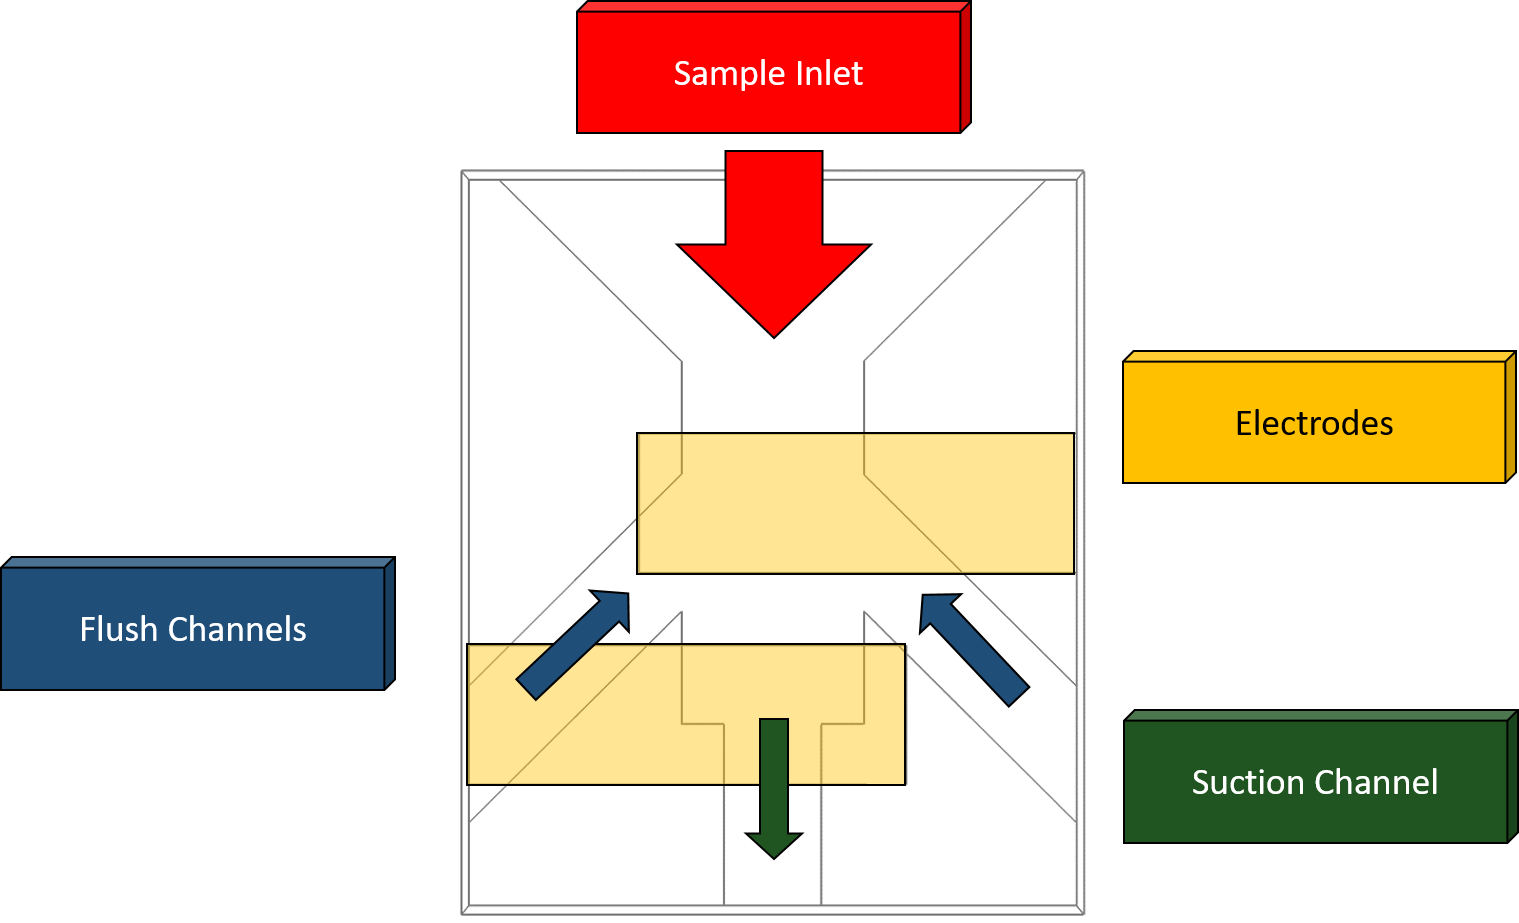
\includegraphics[width=\textwidth]{images/josh_steph_design.png}
    \caption{Functional diagram of cell impedance sensor chamber.}
    \label{fig:josh-steph_functional_diagram}
\end{figure}

\par The impedance sensor was designed with two parallel 11.5 micron wide electrodes with a 5 micron offset that lays under a 15 by 15 micron target measurement area. The device isolates a cell by activating flush and suction channels once a cell from the sample inlet wanders into the test chamber with the purpose of keeping the cell in the test chamber and other cells out (figure \ref{fig:josh-steph_functional_diagram}). Once the device captures a cell, voltage signals over a range of frequencies are applied through the electrodes and the impedance can be calculated from current response.  Figure \ref{fig:josh-steph_sim} depicts the simulated electric fields lines around a cell with desired device behaviour (the development of the COMSOL model is described in section \ref{}). However, the device could not accomplish single-cell isolation and impedance measurements were taken on a suspension of cells (figure \ref{fig:stephanie_impedance_data}).

\begin{figure}[h]
    \centering
    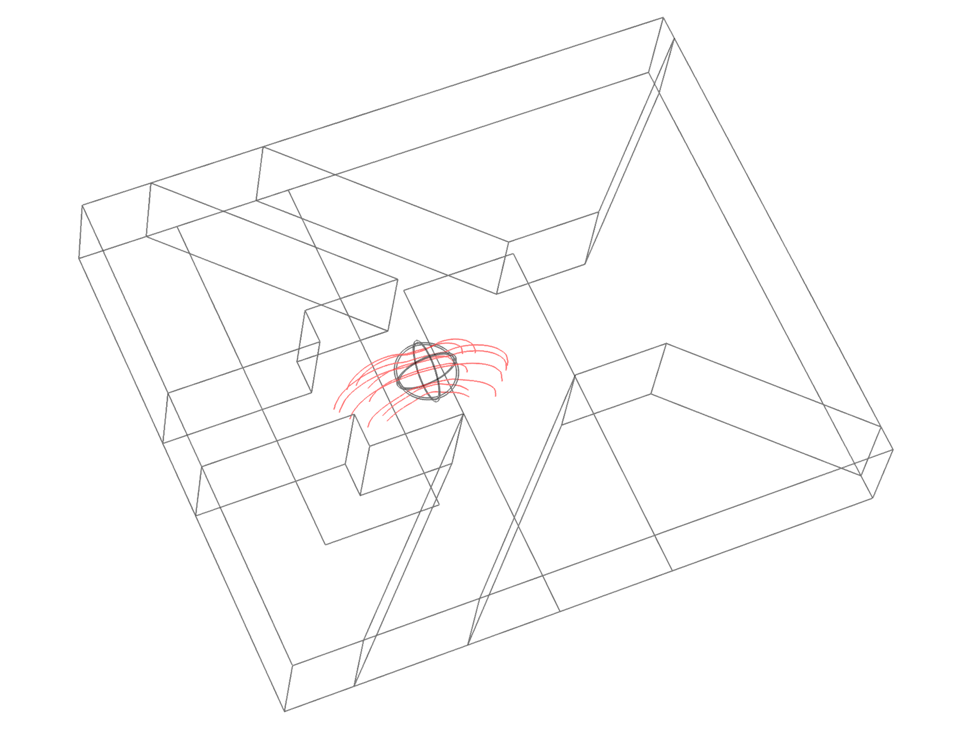
\includegraphics[width=0.9\textwidth]{images/josh_steph_sim.png}
    \caption[Example of desired device behaviour using a COMSOL simulation of electric field lines through a cell.]{Example of desired device behaviour using a COMSOL simulation of electric field lines through a cell. A detailed description of the COMSOL model is presented in section \ref{}}
    \label{fig:josh-steph_sim}
\end{figure}


\begin{figure}[h]
    \centering
    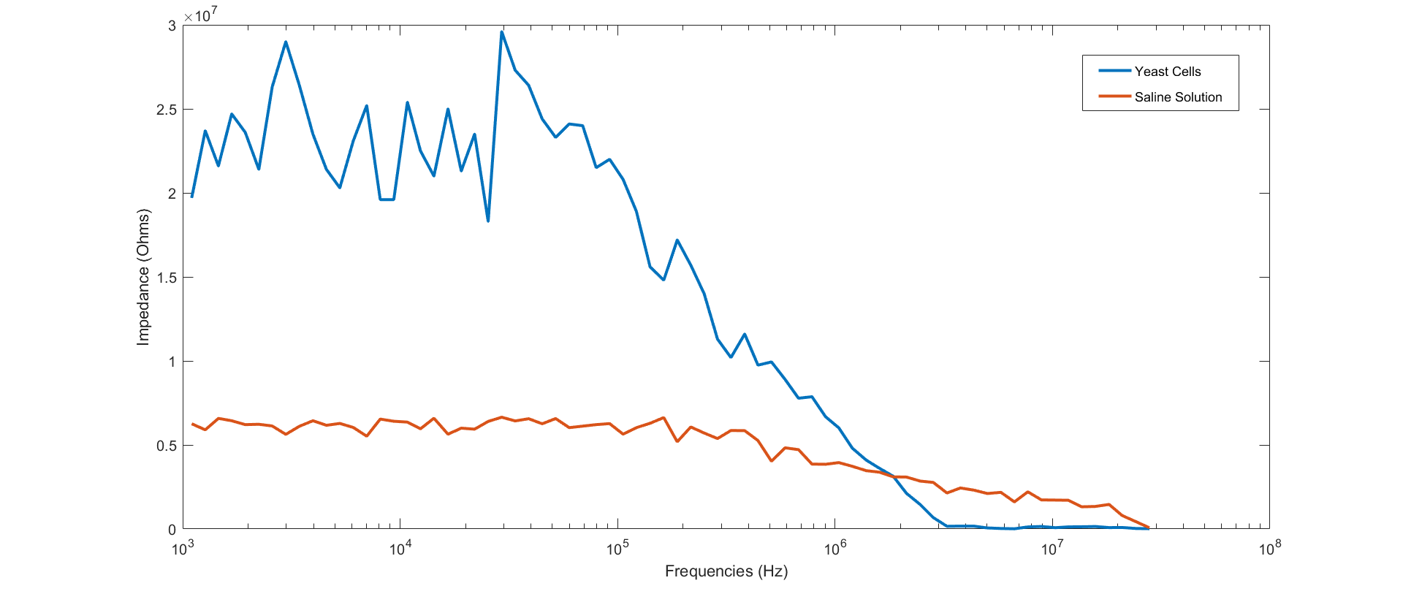
\includegraphics[width=\textwidth]{images/stephanie_impedance_data.png}
    \caption[Impedance spectrum of yeast suspensions and saline solution from the Cal Poly Biofluidic Lab's impedance spectroscopy system]{Impedance spectrum of yeast suspensions and saline solution from the Cal Poly Biofluidic Lab's impedance spectroscopy system \cite{hernandez_single_2009-1}}
    \label{fig:stephanie_impedance_data}
\end{figure}

\par Manufacturing of the device took place in the Cal Poly microfabrication lab and the University of Santa Barbara Nanofabrication Lab. Josh Fadriquela fabricated the microchannels using soft-lithography and Stephanie Hernandez worked the Santa Barbara Lab to create the electrodes with electron beam deposition. Figure \ref{fig:microchannel_mask} and \ref{fig:electrode_mask} depict the masks used in fabricating the microfluidic channels and electrodes.

\begin{figure}[h]
    \centering
    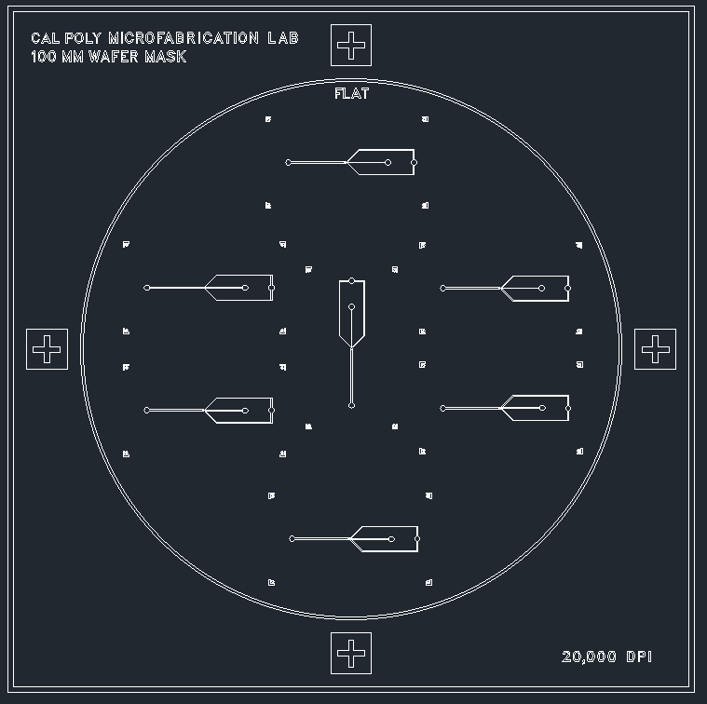
\includegraphics[width=0.6\textwidth]{images/micro_channel_mask.png}
    \caption{Micro channel mask by Josh Fadriquela \cite{fadriquela_design_2009-1}}
    \label{fig:microchannel_mask}
\end{figure}


\begin{figure}[h]
    \centering
    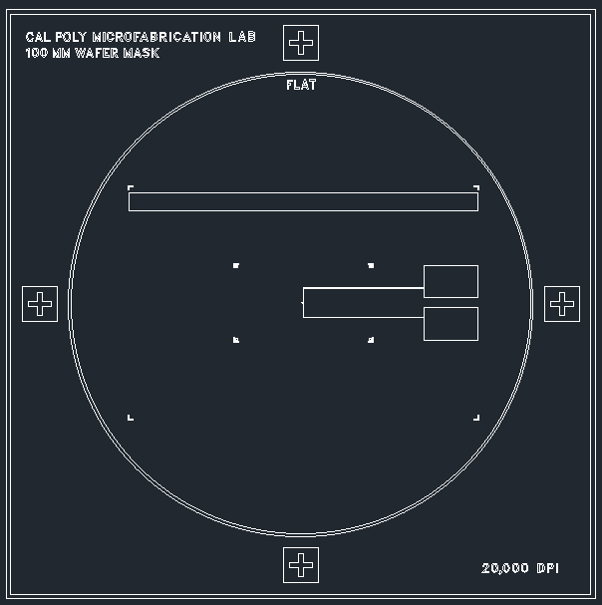
\includegraphics[width=0.6\textwidth]{images/electrode_mask.png}
    \caption{Electrode mask by Stephanie Hernandez \cite{hernandez_single_2009-1}}
    \label{fig:electrode_mask}
\end{figure}

\section[Objectives]{Thesis Purpose and Objectives}

\par The purpose of this thesis is to reevaluate and optimize the Cal Poly Biofluidic Lab's cell impedance spectroscopy system. To accomplish this, the following questions were answered:
\begin{enumerate}
    \item Are there aspects of the impedance spectroscope that need redesign or optimization?
    \item Is the hardware implementation correct?
    \item Can the correct circuit model and desired data acquisition and analysis be packaged and incorporated in a device interface computer program?
    \item Can model based design be applied to characterize and optimize electric fields and impedance to inform future designs?
    \item Can a device be manufactured at Cal Poly to validate the device design and analysis?
\end{enumerate}

\noindent By answering these guiding question, this thesis characterized and enhanced the Biofluidic's Lab's cell impedance spectroscope and provided model validated designs for future IS systems. 